\documentclass[a4paper]{article}

\usepackage[utf8]{inputenc}
\usepackage[T1]{fontenc,url}
\usepackage{cite}
\usepackage{hyperref}
\usepackage{amsmath, amssymb}
\usepackage{tikz}
\usepackage{graphicx}
\usepackage{parskip}
\usepackage{lmodern}
\usepackage{algorithm}
\usepackage{algpseudocode}
\usepackage{epigraph}
\usepackage{listings}
\usepackage{float}



\begin{document}
\title{FYS4150 -- Project 1}
\author{Joachim Falck Brodin,
        Fredrik Jaibeer Mahal Nordeng\\ 
        and Endrias Getachew Asgedom}
    
%\date{September 17, 2016}    % if commented out, the date is set to the current date

\maketitle
\begin{abstract}
\noindent
Numerical methods for solving the one-dimensional Poisson equation with Dirichlet boundary conditions are investigated. In this report, we show how to discretize a one-dimensional Poisson equation and transform it into a linear tridiagonal set of equations. To solve these equations numerically, three different algorithms are developed (i.e., general tridiagonal Gaussian elimination, special tridiagonal Gaussian elimination, and LU-decomposition) and the results are analysed in terms of their computational cost, memory usage, and numerical error. Comparing our numerical solution with the closed form solution, we observe that the numerical approximation error is proportional to the square of the discretization step size, until we experience the loss of precision, due to round off error, when the discretization step size is less then $\sim10^{-5}$. Moreover, the specialized algorithm out performs the two other algorithms in terms of computational cost and memory usage. 
\end{abstract}
\newpage

\tableofcontents

\begin{center}
    GitHub repository at \url{https://github.com/endrias34/FYS4150}
\end{center}

\newpage

%%% MACROS
\newcommand{\half}{\frac{1}{2}}
\newcommand{\dx}{{\Delta x}}
\newcommand{\bigO}{{\mathcal{O}}}


\section{Introduction}
Problems in the field of computational sciences is often formulated in terms of differential equations. Unfortunately, most of these differential equations do not have a closed form solution and hence needs to be solved using numerical methods. In this project, we develop algorithms for a numerical method that solves the one-dimensional Poisson equation with Dirichlet boundary conditions. We use central Finite Difference (FD) method to approximate the second-order differentiation and consequently cast the Poisson equation into a tridiagonal matrix equations. This linear system of equations may be solved using a Gaussian elimination method customized for tridiagonal matrices, also known as Thomas algorithm. Two versions of the Thomas algorithm are considered here; the first assumes a general tridiagonal matrix while the second assumes a Toepliz tridiagonal matrix. As a benchmark, we have also used a more general LU-decomposition method. The accuracy, computational efficiency, and memory usage of the different algorithms are quantitatively analysed.

This report is structured in the following way: First we will briefly present how to discretize the one-dimensional Poisson equation and generate the tridiagonal matrix equations. Second, we will show how to formulate the three different algorithms used to solve the problem. We then analyse the performance of the different algorithms in terms of the number of floating point operations (FLOPs), CPU time, and numerical approximation and precision errors. Finally, we will make a concluding remark.

\section{Theory}
To discretize the one-dimensional Poisson equation and write it in a matrix-vector form, we start with the continuous equation and its corresponding boundary conditions
\begin{equation}
-u''(x) = f(x), \hspace{0.5cm} x\in(0,1), \hspace{0.5cm} u(0) = u(1) = 0,
\label{eq1}
\end{equation}
where $f(x)$ is a known function, called the \textit{source term} and $u(x)$ is a dimension-less physical quantity defined in a dimension-less domain $x$. To solve equation \eqref{eq1} numerically, we first need an approximation of the second derivative of $u$. This can be achieved by performing the Taylor expansion of $u(x)$ around $x$        
\begin{equation}
  u(x\pm h) = u(x) \pm h u^{\prime}(x) + \frac{h^2 u^{\prime\prime}(x)}{2!} \pm  \frac{h^3 u^{\prime\prime\prime}(x)}{3!} + \mathcal{O}(h^4).
\end{equation}

To find an expression containing only the second derivative, we perform the following operation
\begin{equation}
 u(x+h)+u(x-h) = 2u(x) + \frac{2h^2u^{\prime\prime}}{2!} + \mathcal{O}(h^4).
 \label{Ty1}
\end{equation}
We can now solve for $u^{\prime\prime}$ as
\begin{equation}
  u^{\prime\prime}(x) = \frac{u(x+h)+u(x-h)-2u(x)}{h^2} + \mathcal{O}(h^2).
\label{Ty2}
\end{equation}
Notice that the approximation error in equation \eqref{Ty2} is $\mathcal{O}(h^2)$ since we divided \eqref{Ty1} by $h^2$.

For a discrete domain  $x_i=ih$ with $x_0=0$ and $x_{n+1}=1$ as the boundary points, our unknown physical quantity $u$ is represented as $v_i$. Here, the step size is given by $h=1/(n+1)$. The boundary conditions can now be written as $v_0 = v_{n+1} = 0$. Finally, the discrete form of equation \eqref{eq1} is thus given by

\begin{equation}
   -\frac{v_{i+1}+v_{i-1}-2v_i}{h^2} = f_i  \hspace{0.5cm} \mathrm{for} \hspace{0.1cm} i=1,\dots, n,
\label{Eq-DiscEq}
\end{equation}
where $f_i=f(x_i)$ is the discrete version of $f(x)$. To represent equation \eqref{Eq-DiscEq} in a matrix-vector form, we multiply equation \eqref{Eq-DiscEq} with $h^2$ on both sides and write out the equations for all $i$ as follows

\begin{align}
& \color{blue}2*v_1\color{black} - \color{green}1*v_2\color{black} = f_1*h^2\nonumber  \\
&  -\color{red}1*v_1\color{black} + \color{blue}2*v_2\color{black} - \color{green}1*v_3\color{black} = f_2*h^2\nonumber \\
& - \color{red}1*v_2\color{black} + \color{blue}2*v_3\color{black} - \color{green}1*v_4\color{black} = f_3*h^2\nonumber \\ \nonumber\\
  &\vdots \nonumber \\ \nonumber\\
& -\color{red}1*v_{n-2}\color{black} + \color{blue}2*v_{n-1}\color{black} - \color{green}1*v_n\color{black} = f_{n-1}*h^2 \nonumber \\
&  -  \color{red}1*v_{n-1}\color{black} + \color{blue}2*v_n\color{black} = f_n*h^2. 
\label{eq_i}
\end{align}

From equation \eqref{eq_i} we can clearly see how equation \eqref{Eq-DiscEq} can be represented in a matrix-vector form as

\begin{equation}
   \mathbf{A}\mathbf{v} = \tilde{\mathbf{f}},
   \label{mateq1}
\end{equation}
where $\tilde{f}_i\ = f_i*h^2$,
\[
    \mathbf{A} = \begin{bmatrix}
                           \color{blue}2\color{black}& -\color{green}1\color{black}& 0 &\dots   & \dots &0 \\
                           -\color{red}1\color{black} & \color{blue}2\color{black} & -\color{green}1\color{black} &0 &\dots &\dots \\
                           0&-\color{red}1\color{black} &\color{blue}2\color{black} & -\color{green}1\color{black} & 0 & \dots \\
                           & \dots   & \dots &\dots   &\dots & \dots \\
                           0&\dots   &  &-\color{red}1\color{black} &\color{blue}2\color{black}& -\color{green}1\color{black} \\
                           0&\dots    &  & 0  &-\color{red}1\color{black} & \color{blue}2\color{black} \\
                      \end{bmatrix}, \quad \mathbf{v}=\begin{bmatrix}
                           v_1\\
                           v_2\\
                           v_3 \\
                          \dots  \\
                           v_{n-1}\\
                           v_n\\
                      \end{bmatrix} \quad \text{ and } \tilde{\mathbf{f}}=\begin{bmatrix}
                           \tilde{f}_1\\
                           \tilde{f}_2\\
                           \tilde{f}_3 \\
                           \dots \\
                          \tilde{f}_{n-1} \\
                           \tilde{f}_n\\
                      \end{bmatrix}.
\]

Here we can see how each row in the matrix-vector equation corresponds to the sequence of terms as we wrote it out in equation \eqref{eq_i}. We can also observe that $\mathbf{A}$ is tridiagonal matrix. 

\subsection{Gaussian Eliminination for a Tridiagonal Matrix}
Gaussian elimination, or row reduction, is a method for solving a system of linear equations. In the form presented here the procedure is also known as the \textit{Thomas algorithm}. We rewrite our matrix $\mathbf{A}$ in terms of one-dimensional vectors $a,b,c$ and the linear equations can then be presented on the form
\begin{align}
  \begin{bmatrix}
    b_1 & c_1 & 0  & \hdots & \hdots &   0    \\
    a_2 & b_2 & c_2 & 0      & &\vdots \\
    0 & a_3 & b_3  & c_3     & 0 &  \\
    \vdots & 0 & a_4  & b_4     & c_4 & 0 \\
    & & \ddots & \ddots & \ddots & \vdots\\
    0 & \hdots  &\hdots & 0 &a_n & b_n \\
  \end{bmatrix}
  \begin{bmatrix}
    v_1 \\ v_2 \\ v_3 \\ v_4 \\ \vdots \\ \\ v_n
  \end{bmatrix}
  =
  \begin{bmatrix}
    \tilde{f}_1 \\ \tilde{f}_2 \\ \tilde{f}_3 \\ \tilde{f}_4 \\ \vdots \\ \\ \tilde{f}_n
  \end{bmatrix}.
  \label{eqg1}
\end{align}
Next, we eliminate the $a_2$ from the second row. Here, the first step is to subtract $\frac{a_2}{b_1}$ times the first row from the second row and obtain
\begin{align}
  \begin{bmatrix}
    b_1 & c_1 & 0  & \hdots & \hdots &   0    \\
    0 & b'_2 & c_2 & 0      & &\vdots \\
    0 & a_3 & b_3  & c_3     & 0 &  \\
    \vdots & 0 & a_4  & b_4     & c_4 & 0 \\
    & & \ddots & \ddots & \ddots & \vdots\\
    0 & \hdots  &\hdots & 0 &a_n & b_n \\
  \end{bmatrix}
  \begin{bmatrix}
    v_1 \\ v_2 \\ v_3 \\ v_4 \\ \vdots \\ \\ v_n
  \end{bmatrix}
  =
  \begin{bmatrix}
    \tilde{f}_1 \\ \tilde{f}'_2 \\ \tilde{f}_3 \\ \tilde{f}_4 \\ \vdots \\ \\ \tilde{f}_n
  \end{bmatrix},
  \label{eqg2}
\end{align}
where $b'_2 = b_2 - \frac{a_2}{b_1} c_1$ and $\tilde{f}'_2 = \tilde{f}_2 - \frac{a_2}{b_1}\tilde{f}_1$. For the following rows we proceed in the same manner and we can generally express the different rows as
\begin{equation}
  b'_i = b_i - \frac{a_i}{b'_{i-1}}c_{i-1},
  \label{forward1}
\end{equation}
with $b'_1 = b_1$, and
\begin{equation}
  \tilde{f}'_{i} = \tilde{f}_i - \frac{a_i}{b'_{i-1}}\tilde{f}'_{i-1},
  \label{forward2}
\end{equation}
where $\tilde{f}'_1 = \tilde{f}_1$. Finally, the system of equations become an upper triangular matrix equation of the form
\begin{equation}
  \begin{bmatrix}
    b'_1 & c_1 & 0  & \hdots & \hdots &   0    \\
    0 & b'_2 & c_2 & 0      & &\vdots \\
    0 & 0 & b'_3  & c_3     & 0 &  \\
    \vdots & 0 & 0  & b'_4     & c_4 & 0 \\
    & & \ddots & \ddots & \ddots & \vdots\\
    0 & \hdots  &\hdots & 0 &0 & b'_n \\
  \end{bmatrix}
  \begin{bmatrix}
    v_1 \\ v_2 \\ v_3 \\ v_4 \\ \vdots \\ \\ v_n
  \end{bmatrix}
  =
  \begin{bmatrix}
    \tilde{f}'_1 \\ \tilde{f}'_2 \\ \tilde{f}'_3 \\ \tilde{f}'_4 \\ \vdots \\ \\ \tilde{f}'_n
  \end{bmatrix}.
  \label{eqg3}
\end{equation}
The process of converting the matrix equation from \eqref{eqg1} to \eqref{eqg3} is known as $forward$ $substitution$. To find the solution $v_i$ for the matrix equation \eqref{eqg3}, we can start from the bottom and solve for $v_n$, then continue to solve for $v_{n-1}$ until we reach $v_0$. This way of solving the matrix equation is known as $backward$ $substitution$ and it can be generalized to

\begin{equation}
    v_i =
    \begin{cases}
      \tilde{f}'_n/b'_n, & \text{if}\ i=n \\
      (\tilde{f}'_i- c_i v_{i+1})/b'_i, & \text{otherwise}.

    \end{cases}
    \label{backward1}
  \end{equation}

\subsection{Gaussian Elimination for a Toepliz Tridiagonal Matrix}
Matrix $\mathbf{A}$ in equation \eqref{mateq1} has a Toepliz tridiagonal structure. This means the non-zero diagonal elements have the same value along all the diagonal. In our case, we have $a_i = c_i = -1$ and $b_i = 2$. The fact that the elements of matrix $\mathbf{A}$ only have two different values greatly simplifies the Gaussian elimination method discussed in the previous section. The forward substitution step in equations \eqref{forward1} and \eqref{forward2} can now be generalized to
\begin{equation}
  b'_i = \frac{i+1}{i}, \qquad i=1,\dots,n-1,
  \label{simple1}
\end{equation}
and
\begin{equation}
  \tilde{f}'_{i} = \tilde{f}_i + \frac{\tilde{f}'_{i-1}}{b'_{i-1}}, \qquad i=1,\dots,n-1.
  \label{simple2}
\end{equation}
Similarly, the backward substitution step in equation \eqref{backward1} simplifies to
\begin{equation}
  v_i = \frac{\tilde{f}'_i +  v_{i+1}}{b'_i} \qquad i=n-2,n-1,\dots,0.
  \label{simple3}
\end{equation}
\subsection{LU-decomposition Method}
The LU-Decomposition method is the most commonly used method to solve a linear system of equation which has a densely populated matrix. The method is a special form of Gaussian elimination method and considers we have a non-singular matrix $\mathbf{A}$ that can be decomposed into a product of two triangular matrices $\mathbf{L}$ and $\mathbf{U}$, where $\mathbf{L}$ is a lower-triangular matrix with all diagonal entries equal to $1$ and $\mathbf{U}$ is an upper-triangular matrix. To solve the linear set of equation $\mathbf{A}\mathbf{v} = \mathbf{\tilde{f}}$ using LU-decomposition, we substitute $\mathbf{A} = \mathbf{L}\mathbf{U}$  such that
\begin{equation} 
 \mathbf{L}\mathbf{U}\mathbf{v} = \mathbf{L}\mathbf{y} = \mathbf{\tilde{f}},
 \label{lu1}
\end{equation}
where $\mathbf{y}=\mathbf{U}\mathbf{v}$. Consequently, the solution $\mathbf{v}$ can now be obtained by solving the following two triangular linear set of equations
\begin{equation} 
\begin{split}
 \mathbf{L}\mathbf{y} &= \mathbf{\tilde{f}} \\
 \mathbf{U}\mathbf{v} &= \mathbf{y}.
\end{split}
 \label{lu2}
\end{equation}
Solving triangular set of equations is trivial, as the lower triangular equation can be solved using $forward$ $substitution$ while the upper triangular equation may be solved by $backward$ $substitution$.

\section{Method}
The three different algorithms required to solve the tridiagonal matrix equation are implemented using C++ and the corresponding source codes can be found in the github repository address linked to this report. In this section, we outline the algorithms structure using pseudo-codes, discuss about the FLoating point OPerations (FLOPs) counts, and the memory handling of each of the algorithms.  
 
\subsection{General Tridiagonal Matrix Algorithm}
The algorithm we will present here is known as the Thomas algorithm. The main elements of the algorithm are the $forward$ and $backward$ substitution (see Algorithm \eqref{algo-thom1}). The algorithm take the vectors $\mathbf{a}\in\mathbb{R}^{n-1}$,$\mathbf{b}\in\mathbb{R}^{n}$,$\mathbf{c}\in\mathbb{R}^{n-1}$, and $\mathbf{\tilde{f}}\in\mathbb{R}^{n}$ as input and outputs the solution $\mathbf{v}\in\mathbb{R}^{n}$. Notice that we do not reserve storage for the full $\mathbf{A}\in\mathbb{R}^{n\times n}$ matrix, but rather only store the nonzero tridiagonal elements as vectors. This allows us to utilize this algorithm for solving problems with a very large number of $n$ without running into a memory allocation problem.

\begin{algorithm}[H]
\caption{General Tridiagonal Matrix Algorithm}\label{algo-thom1}
\textbf{Input:} $\mathbf{a}, \mathbf{b},\mathbf{c},\mathbf{\tilde{f}}$ \\
\textbf{Output:} $\mathbf{v}$
\begin{algorithmic}[1]
\State $b'_0=b_0$ \qquad// First element along main diagonal
\State $\tilde{f}'_0=\tilde{f}_0$ \qquad// First element in the RHS\\
    \State // Forward substitution
	\For {$i=1$ to $i=n-1$}
		\State $b'_i=b_i-a_{i-1}*c_{i-1}/b'_{i-1}$	\qquad// Eliminate lower diag	  
		\State $\tilde{f}'_i=\tilde{f}-a_{i-1}*\tilde{f}_{i-1}/b'_{i-1}$  \qquad// Change RHS
	\EndFor \\
    
    \State // Backward substitution
    \State $v_{n-1}=\tilde{f}'_{n-1}/b'_{n-1}$ \qquad\qquad// Final element of the solution\\
    \For {$i=n-2$ to $i=0$}
		\State $v_i=(\tilde{f}'_{i}-c_i*v_{i+1})/b'_i$ 
	\EndFor 
\end{algorithmic}
\end{algorithm}

The number of FLOPs for the Thomas algorithm is composed of $6(n-1)$ for the forward and $3(n-1)$ for the backward substitution. Moreover, pre-computing $a_{i-1}/b'_{i-1}$ (cf. line $6$ and $7$ in Algorithm \ref{algo-thom1}) in the forward substitution, we can reduce the number of FLOPs by $(n-1)$. Therefore, in total the Thomas algorithm requires $8(n-1)$ FLOPs.

\subsection{Toepliz Tridiagonal Matrix Algorithm}
The Toepliz structure of matrix $\mathbf{A}$ allows us to reduce both the memory demand and the FLOPs of the Thomas algorithm. This specialized form of the Thomas algorithm takes only $\mathbf{\tilde{f}}\in\mathbb{R}^{n}$ as input and outputs the solution $\mathbf{v}\in\mathbb{R}^{n}$. Similarly, the FLOPs reduce to $2(n-1)$ for the forward and another $2(n-1)$ for the backward substitution. The reduction in the forward substitution is due to the fact that the diagonal elements in line $6$ of algorithm \ref{algo-thom2} can now be fully precomputed since they have analytical expression. Therefore, the total FLOPs for the specialized Thomas algorithm is $4(n-1)$ which is a reduction by half compared to the general Thomas algorithm. 

\begin{algorithm}[H]
\caption{Toepliz Tridiagonal Matrix Algorithm}\label{algo-thom2}
\textbf{Input:} $\mathbf{\tilde{f}}$ \\
\textbf{Output:} $\mathbf{v}$
\begin{algorithmic}[1]
\State $b'_0=2$ \qquad// First element along main diagonal
\State $\tilde{f}'_0=\tilde{f}_0$ \qquad// First element in the RHS\\ 

    \State // Forward elimination
	\For {$i=1$ to $i=n-1$}
		\State $b'_i=(i+2)/(i+1)$ \qquad// Eliminate lower diag
		\State $\tilde{f}'_i=y_i+\tilde{f}_{i-1}/b'_{i-1}$ \qquad// Change RHS
	\EndFor \\
    \State // Backward elimination
    \State $v_{n-1}=\tilde{f}'_{n-1}/b'_{n-1}$ \qquad\qquad// Final element in solution
    \For {$i=n-2$ to $i=0$}
		\State $v_i=(\tilde{f}'_{i}+v_{i+1})/b'_i$ 
	\EndFor
\end{algorithmic}
\end{algorithm}

\subsection{LU-decomposition based Toepliz Tridiagonal Matrix Algorithm}
Here, we used $Armadillo$ (a C++ Linear Algebra Library \cite{Arma}) to perform LU-decomposition and solve the Toepliz triangular set of linear equations. Armadillo has a built in function called $solve$ that is a highly optimized function that performs LU-decomposition by default to solve a linear set of equations. However, in our pseudo-code (cf. algorithm \ref{alg:LU}) we have separately specified the LU-decomposition and solving the two triangular equations for clarity of presentation. Any LU-decomposition based algorithm is composed of three steps; first LU-decomposition of the system matrix, and then triangular forward substitution, and at last triangular backward substitution. The pseudo-code in algorithm \ref{alg:LU} takes as input $\mathbf{A}\in\mathbb{R}^{n\times n}$ and $\mathbf{\tilde{f}}\in\mathbb{R}^{n}$, and outputs the solution $\mathbf{v}\in\mathbb{R}^{n}$. Here, it is pertinent to note that algorithm \ref{alg:LU} takes a matrix as input, and hence requires a large amount of memory to store this matrix. Nevertheless, LU-decomposition is a method of choice when solving a linear set of equation with a densely populated matrix. For the case $\mathbf{A}\in\mathbb{R}^{n\times n}$, the FLOPs for LU-decomposition takes $O(2/3n^3)$, and the two substitutions take each $\sim O(n^2)$ \cite{Comp}. However, here we are interested in solving a system of equations with a Toepliz tridiagonal matrix structure. For such a case the LU-decomposition has an analytical expression and takes only $O(3n)$ FLOPs, the forward substitution takes $O(2n)$ while the backward substitution takes $O(3n)$ \cite{PresTeukVettFlan92}. In total the number of FLOPs for LU-decomposition based Toepliz tridiagonal matrix system of equations is $8n$.

\begin{algorithm}[H]
\caption{LU-decomposition based Toepliz Tridiagonal Matrix Algorithm}\label{alg:LU}
\textbf{Input:} $\mathbf{\tilde{A}}$ and $\mathbf{\tilde{f}}$ \\
\textbf{Output:} $\mathbf{v}$
\begin{algorithmic}
	\State $lu(L,U,A)$ \      \qquad// LU-decomposition 
    \State $y = solve(L,\tilde{f})$ \ \qquad// Forward substitution 
    \State $v = solve(U,y)$ \ \qquad// Backward substitution 
\end{algorithmic}
\end{algorithm}

\subsection{Error Analysis}
The error generated by the different algorithms developed in this project are quantified by comparing the results of the algorithm with that of the closed form (analytical) solution using the relative error defined by
\begin{equation}
  \epsilon_i = \left|\frac{v_i^{num} - v_i^{ana}}{v_i^{ana}}\right|, \quad i=1,\dots,n,
  \label{rerr}
\end{equation}
where $v_i^{num}$ and $v_i^{ana}$ are the numerical and analytical solutions at the $i^{th}$ descritization location, respectively. Moreover, $\left|.\right|$ is the absolute value operator. The analytical solution for the one-dimensional Poisson equation with a known source function is derived in Appendix \ref{ana-sol}.
  
\section{Results}

\subsection{Computational Time}
To compare the computational efficiency of the three different algorithms discussed in this project we analysed their execution time elapsed in terms of CPU time (cf. Tabel \ref{CPU}). The time is computed by taking an average of $1000$ runs of each of the algorithms. Considering the number of FLOPs count for the three different algorithms, one might expect to see the CPU time for LU-decomposition and general Thomas algorithm to be similar while the special Thomas algorithm being twice faster than the two other algorithms. However, what we actually observe from the CPU time is that the special Thomas algorithm is slightly faster than the general Thomas algorithm and the LU-decomposition algorithm is at least an order of magnitude slower then the two Thomas algorithms. Another observation that we can make from the CPU time is that, as the matrix size gets larger the special Thomas algorithm gets more faster than the general Thomas algorithm. Furthermore, the CPU time difference between the two Thomas algorithms and the LU-decomposition reduces as the matrix size gets larger.

\begin{table}[ht]
%\caption{Timing our code}
\begin{center}
  \begin{tabular}{| l | l | l | l |}
  \hline
    Matrix size &  General [s] & Special [s] & LU-decomp. [s]\\[0.10cm]\hline\hline
     & & & \\
     $10\times10$ & $6.970\cdot10^{-7}$ & $6.910\cdot10^{-7}$ & $1.139\cdot10^{-5}$\\[0.10cm]
    $100\times100$ & $2.114\cdot10^{-6}$ & $2.047\cdot10^{-6}$& $6.882\cdot10^{-5}$\\[0.10cm]
     $1000\times1000$ & $1.676\cdot10^{-5}$& $1.577\cdot10^{-5}$& $2.722\cdot10^{-4}$\\[0.10cm]
     \hline
  \end{tabular}
\end{center}
\caption{CPU time in seconds for the three different algorithms (i.e., General and special Thomas, and LU-decomposition).}
\label{CPU}
\end{table}

One possible reason for explaining the discrepancy between the FLOPs count and the CPU time is that, not all operations consume the same CPU time. For example it is known that division is the most computationally costly operation. Thus, comparing the two Thomas algorithms, it is possible to see that the number of division operations are the same. Therefore, it might be possible that the division operation is the cause for not seeing the special algorithm not being twice as fast as the general algorithm. On the other hand, the very slow LU-decomposition algorithm could be because Armadillo might have treated the matrix $\mathbf{A}$ as a fully populated matrix.

\subsection{Algorithm Benchmark and Error Analysis}
Due to the availability of the analytical solution to the one-dimensional Poisson equation, we have bechmarked our numerical algorithms by computing the relative error. We considered three different cases (i.e., $n=10$, $n=100$, and $n=1000$) and show the results only for the general Thomas algorithm. This is mainly because the two other algorithms provide a similar result as that of the general Thomas algorithm. Figure \ref{fig1} presents the numerical solution for the three different cases as well as the corresponding analytical solution. Here, we can observe that for the cases $n=100$ and $n=1000$ the numerical solution is the same as the analytical solution. To quantify the difference between the numerical and analytical solutions, we computed the relative error for the three different cases and shown it in logarithmic scale in Figure \ref{fig2}. Notice that the relative error is the same for all values of $x$ and that for $n=10$, $\epsilon \sim 10^{-1.2}$, for $n=100$, $\epsilon \sim 10^{-3}$, and for $n=1000$, $\epsilon \sim 10^{-5}$.

\begin{figure}[H]
  \centering
  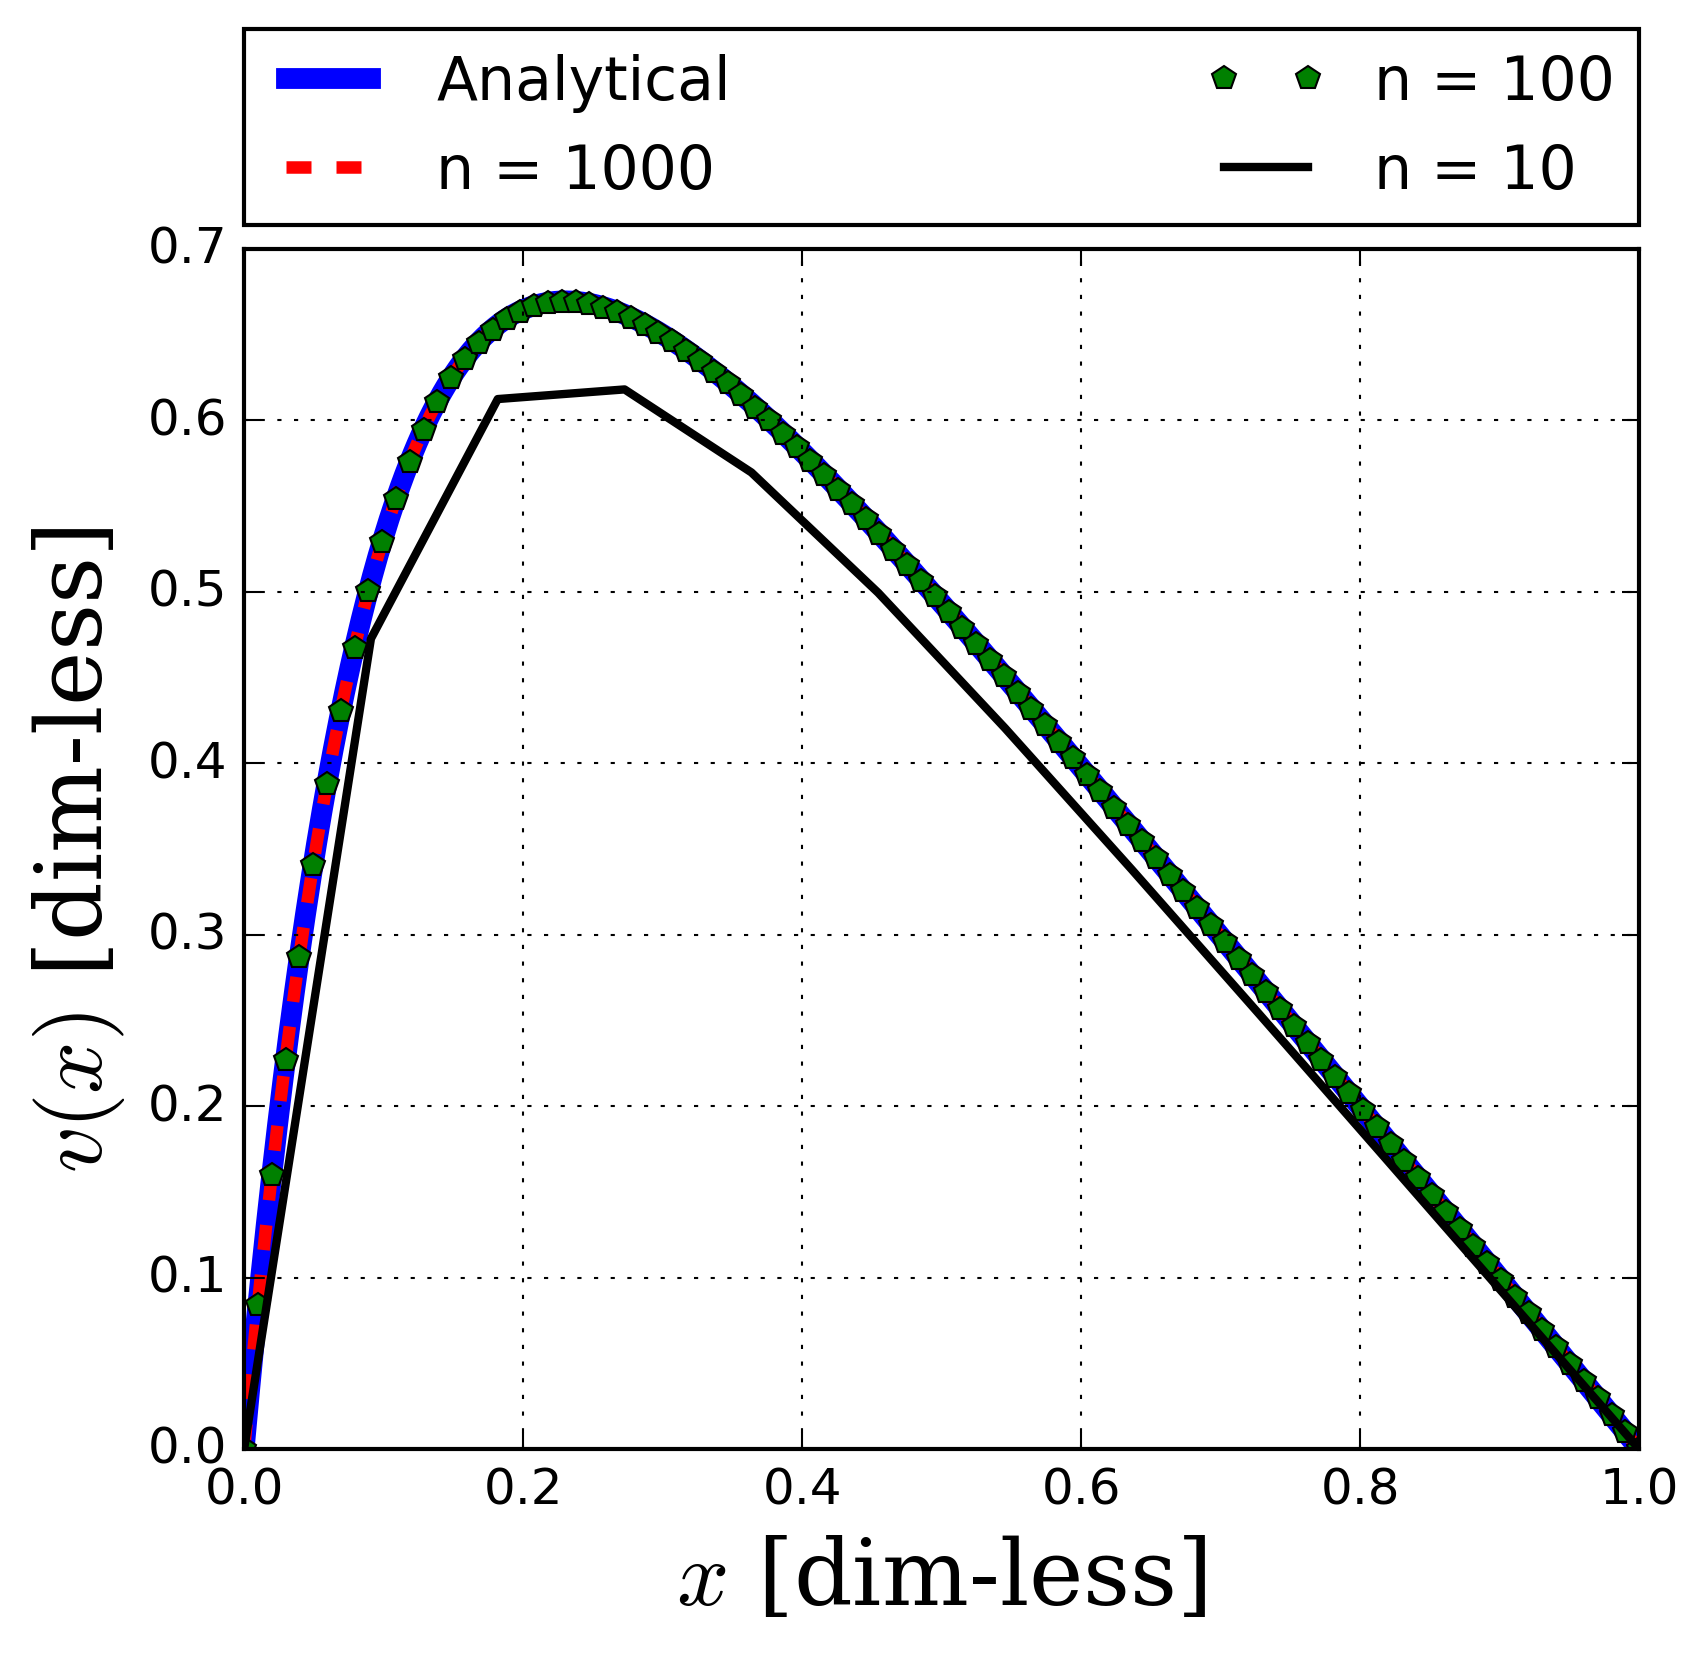
\includegraphics[width=\columnwidth]{Results_general.png}
  \caption{Numerical approximation and analytical solution to the 1D Poisson equation. The numerical solution is shown for different $n \times n$ matrix sizes. The convergence of the numerical method is
    apparent as its graph approaches the analytical solution as the number of points \(n\) grows. When \(n
    >= 10^{2}\), the numerical solution becomes indistinguishable from the analytical solution.}
    \label{fig1}
\end{figure}

\begin{figure}[H]
  \centering
  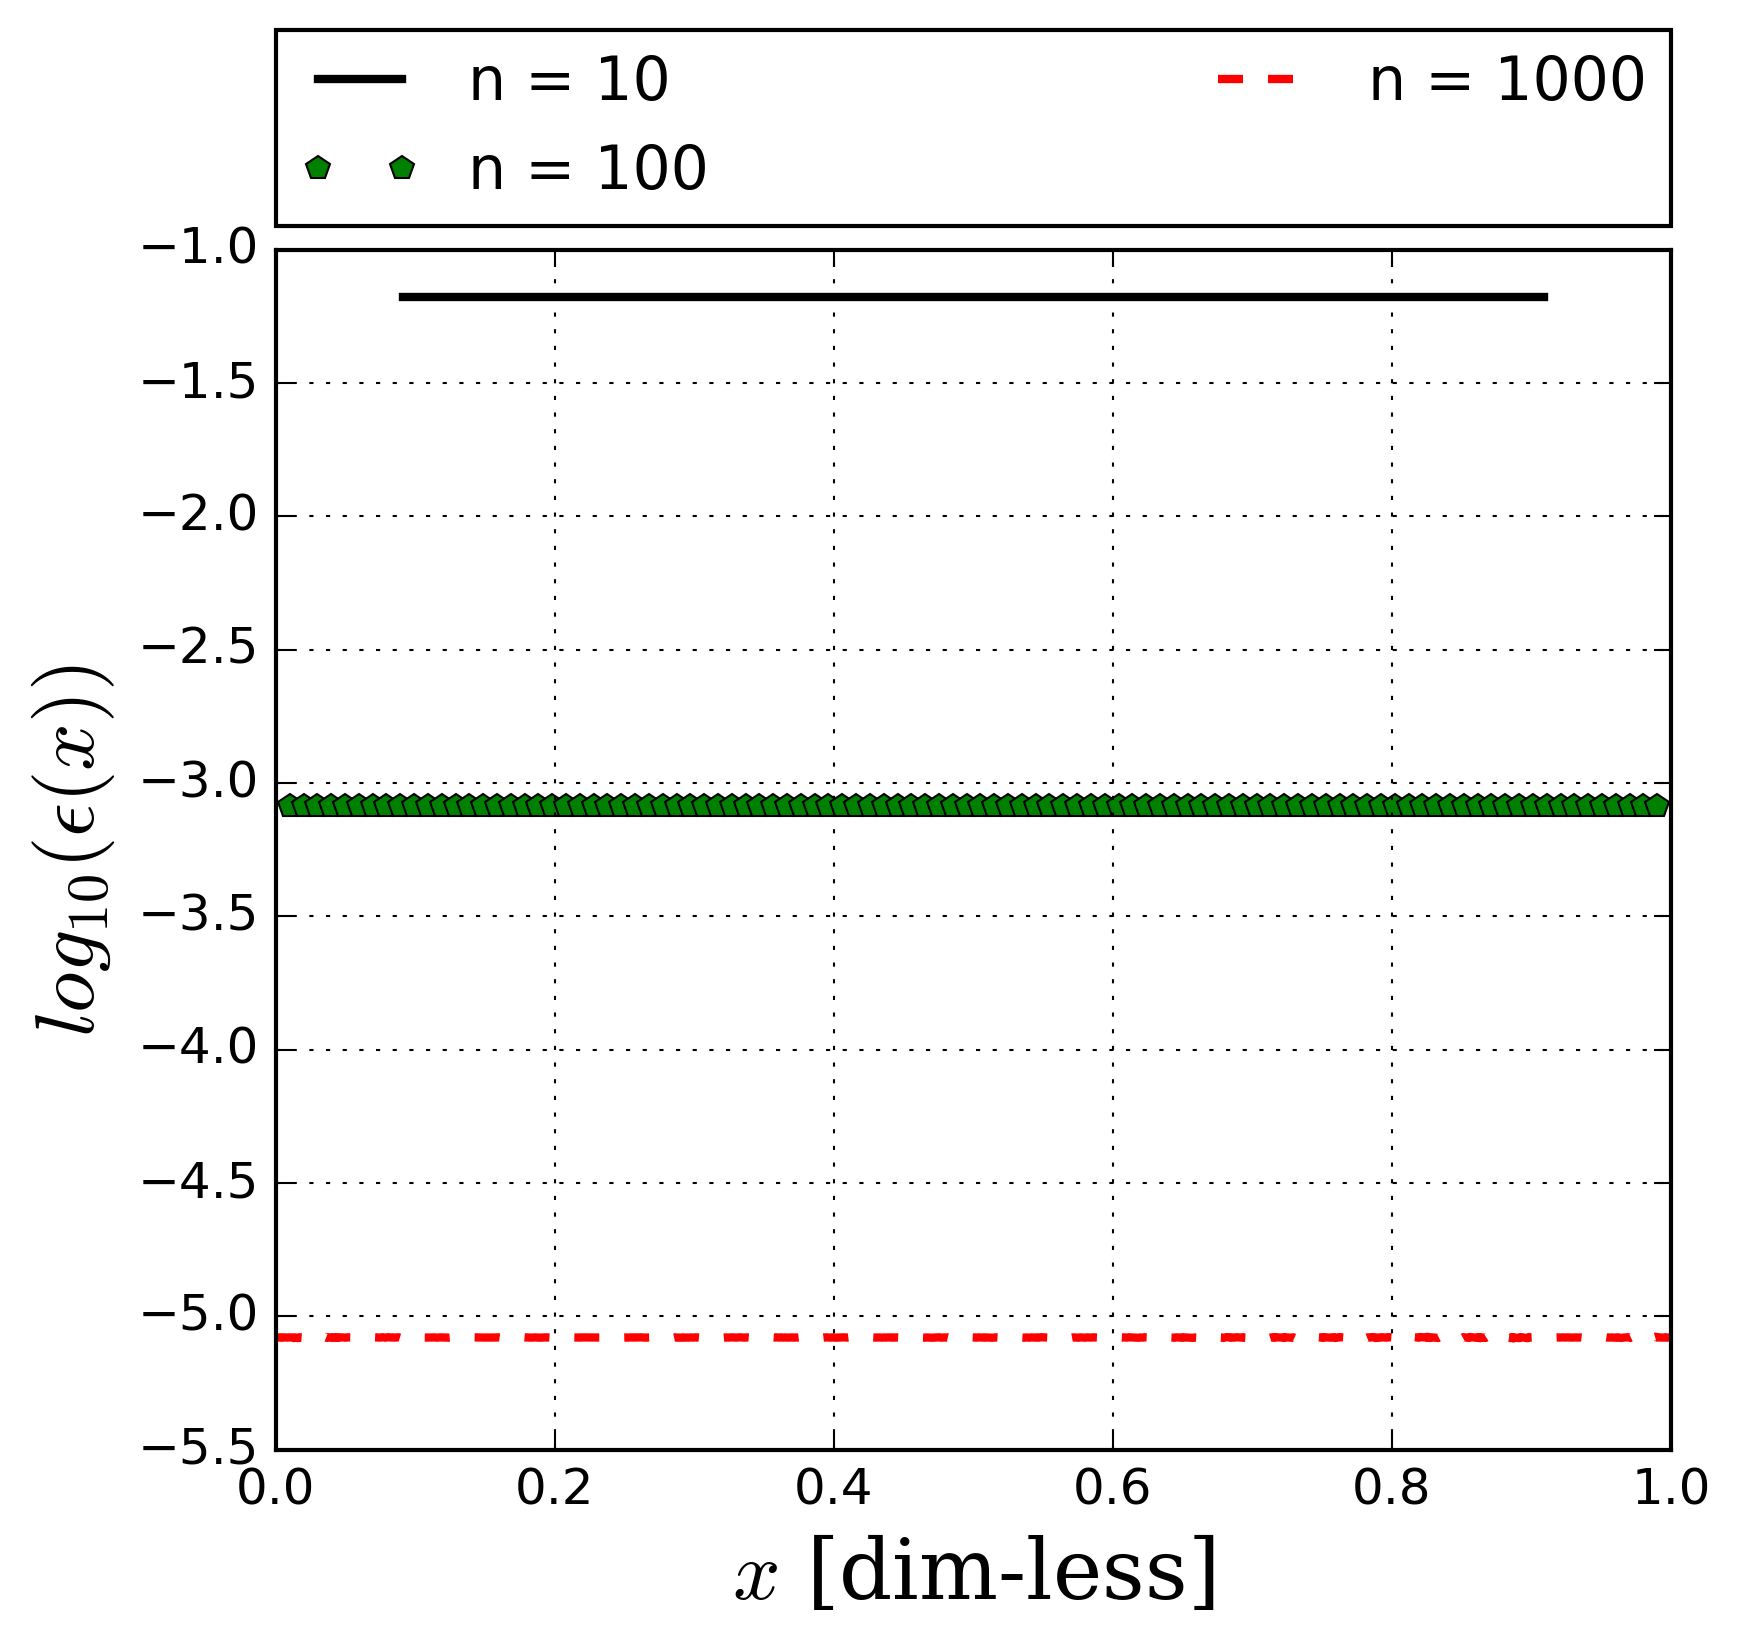
\includegraphics[width=\columnwidth]{RelativeError_general.png}
  \caption{ Relative error to the numerical approximations of the 1D Poisson equation. The relative error is shown for different $n \times n$ matrix sizes.}
  \label{fig2}
\end{figure}

To analyse the effect of having extremely small descritization step size (or  having very large number of grid points $n$) on the precision of the numerical algorithm, we computed the relative error for the general Thomas algorithm for different values of descritization step sizes (cf. Tabel \ref{RelativErr} and Figure \ref{fig3}). The logarithmic relative error as a function of the logarithmic descritization step size shows a linear trend and it reduces until it reaches a descritization step size of $\sim 10
^{-5}$ (or $n=10^{5}$), where it increases again. This loss of precision is due to round off errors which arises from the fact that computers do not represent numbers with an infinite decimal places and hence need to be rounded off to a number the computer can represent. 

\begin{table}[H]
\begin{center}
  \begin{tabular}{| l | l |l |}
  \hline
    Grid points ($n$) & Step size ($log_{10}(h)$) & Relative error ($log_{10}(\epsilon)$)  \\[0.10cm]\hline \hline
     & \\
     $10^1$ & $-1.041$ & $  -1.179  $ \\[0.10cm]
     $10^2$ & $-2.004$ & $  -3.0880 $ \\[0.10cm]
     $10^3$ & $-3.000$ & $  -5.0807 $ \\[0.10cm]
     $10^4$ & $-4.000$ & $  -7.0791 $ \\[0.10cm]
     $10^5$ & $-5.000$ & $  -8.843  $ \\[0.10cm]
     $10^6$ & $-6.000$ & $  -6.075  $ \\[0.10cm]
     $10^7$ & $-7.000$ & $  -5.525  $ \\[0.1cm]
     \hline
  \end{tabular}
\end{center}
\caption{Logarithmic relative error as a function of logarithmic discretization step size (or the number of grid points). Here we have calculated the maximum relative error for each of the discretization step sizes.}
\label{RelativErr}
\end{table}

\begin{figure}[H]
  \centering
  \includegraphics[width=\columnwidth]{precision_general.png}
  \caption{\label{fig:prec} A plot of the logarithmic relative error as a function of the logarithmic disretization step size. Here we can see that the relative error follows our expectation for the truncation error, with a slope value of -2 on a logarithmic scale, up to a point of $n\sim 10^5$.}
  \label{fig3}
\end{figure}

\section{Discussion}
The memory usage of the three different algorithms depends on whether the algorithm uses static or dynamic memory allocation. In addition, it also depends whether the algorithm has to store vectors or matrices. In this project we have allocated all our variables using dynamic memory. It is also important to notice that the LU-decomposition algorithm has to store a matrix while the two Thomas algorithms store only vectors. Consequently, we would run into a memory storage problem when using the LU-decomposition algorithm. For example, consider a problem with the number of grid points $n=10^5$. This implies matrix $\mathbf{A}\in\mathbb{R}^{10
^5\times 10^5}$. To store this matrix in memory requires $10^{10}*64/(8\cdot 10^9)=80$GB for double precision numbers. Unfortunately, this is by far larger than a normal personal computer memory ($\sim 8$GB). 

\section{Conclusion}
Three different numerical algorithms were developed for solving the one dimensional Poisson equation with Dirichlet boundary conditions. The algorithms utilize the fact that the problem can be casted into a matrix equation. The general Thomas algorithm uses the tridiagonal structure of the matrix equation while the special Thomas and LU-decomposition algorithms use the Toepliz tridiagonal structure for the matrix $\mathbf{A}$. This allows the three algorithms to be computationally efficient compared to the general Gaussian elimination algorithm. Moreover, the results of the three algorithms approach the corresponding analytical solution with a small relative error for the number of grid points $n \geq 100$. The special Thomas algorithm out performed the two other algorithms by having the fastest computational speed and the smallest memory requirement. The LU-decomposition algorithm has the highest memory requirement and it was even impossible to use the method in a personal computer for $n > 10^{4}$. Finally, we have observed that the numerical precision of the algorithms increases with in creasing the $n$ until it reaches the round off limit $n \sim 10^{5}$.\\

%\bibliographystyle{plain}
%\bibliographystyle{siam}
\bibliography{sample}
\bibliographystyle{IEEEtran}

\begin{appendix}
\section{Analytical Solution}
\label{ana-sol}
The one-dimensional Poisson equation with Dirichlet boundary condition has a closed form solution for a known and twice integrable source function. To derive this closed form solution, we first rewrite equation \eqref{eq1} for a source function $f(x) = 100 e^{-10x}$ as
\begin{align}
  -u''(x) = 100 e^{-10x}, \hspace{0.5cm} x\in(0,1), \hspace{0.5cm} u(0) = u(1) = 0.
  \label{eqA1}
\end{align}
A closed form solution to equation \eqref{eqA1} can now be found by integrating it twice respect to $x$. This results 
\begin{align}
  u(x) = -e^{-10x} + A + Bx,
  \label{eqA2}
\end{align}
where $A$ and $B$ are integration constants. We now impose the Dirichlet boundary condition to equation \eqref{eqA2} and find that $A=1$ and $B=e^{-10}-1$. Finally, replacing the values of $A$ and $B$ into equation \eqref{eqA2} results the analytical solution
\begin{align}
  u(x) = 1 - (1 - e^{-10})x - e^{-10x}.
\end{align}
\end{appendix}
\end{document}
